\section{Application to a real TLP generator}
\label{sec:tlp-modeling}

The methodology described in section \ref{sec:esd-modeling} is applied to the \gls{tlp} bench at NXP laboratory in Toulouse.
The model is validated by comparing simulations with measurements of current and voltage waveforms at different charging voltages and on different loads.
The complete model is detailed Fig. \ref{fig:complete-tlp-model}.
A few elements in it are specific to the simulation, but overall most of them physically exist.
Initially, the relay is left open.
The 50 ns coaxial cable on the left is charged by the high voltage\gls{dc} supply.
The 10 M\textOmega resistor serves two purposes.
It ensures that the cable charges slowly to avoid oscillations.
Also, it isolates the high voltage supply from the discharge when it is triggered.
The two $1 fF$ capacitors placed at each end of the discharge cable help the simulator to set a charging voltage as initial condition.
After the relay, a 50\textOmega resistor can be found, that was used as poor-man's attenuator.
Despite having a value of 50\textOmega like the coaxial cables, this resistor creates an impedance mismatch that strongly impacts the waveforms.
A current probe is found immediately after the attenuator.
A voltage probe is connected
Current and voltage probe locations are important to align the waveforms.
Because of the delays, waveforms are shifted in time compared to one another.
Between the two probes, a few short transmission lines are found.
They correspond to short coaxial cablse inside the testbench.
Finally, two discharge paths are possible inside the generator depending on the configuration of the switch on the output.
The direct path is on the bottom, and the top path provides a series resistance to limit the discharge current.

\begin{figure}[!h]
  \centering
  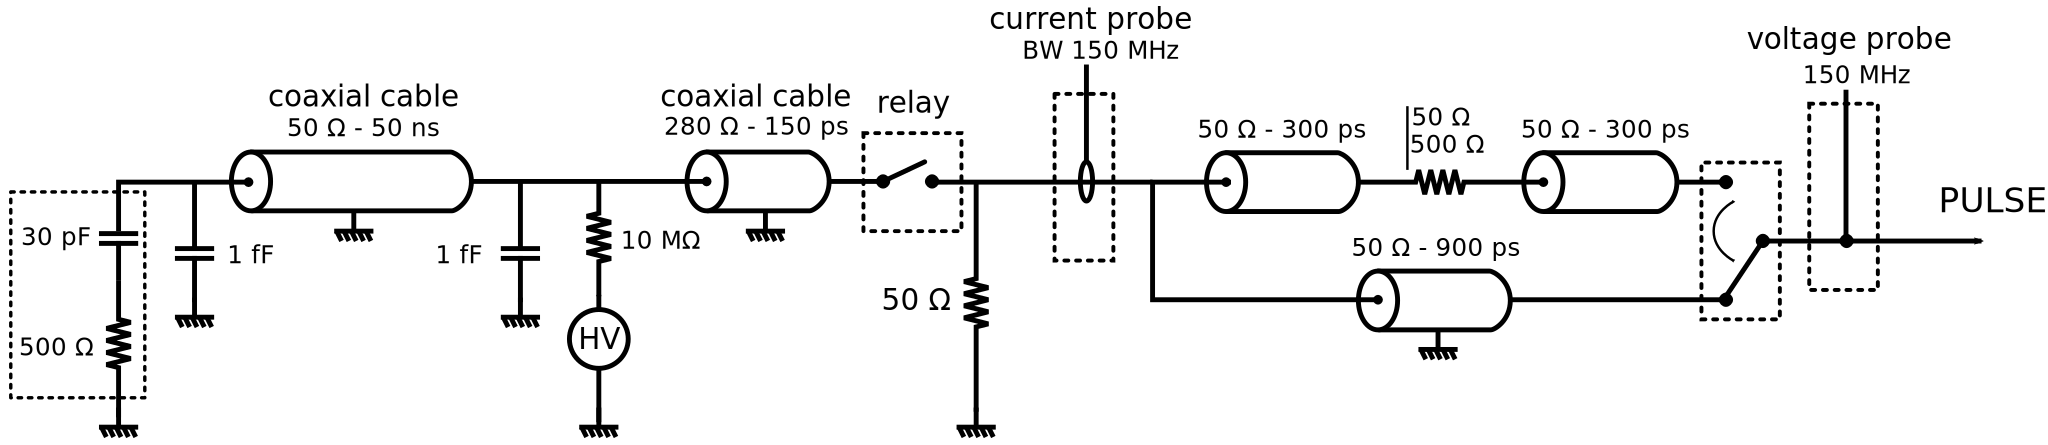
\includegraphics[width=\textwidth]{src/2/figures/complete_nxp_tlp_model.pdf}
  \caption{Complete model of NXP laboratory's TLP generator}
  \label{fig:complete-tlp-model}
\end{figure}

%TODO: next
% TODO: is it correct the value
Simulation and measurement curves for each load are given at 3.5 A, corresponding to a 500 V TLP charging voltage and a XXX\textOmega load.
Curves at 75 mA (10 V) and 7.5 A (1000 V) will be given in annex ?

% What conditions for the characterization setup
The setup is identical for each simulation and measurement and is given Fig. \ref{fig:setup-cz-tlp-model}.

\begin{figure}[!h]
  \centering
  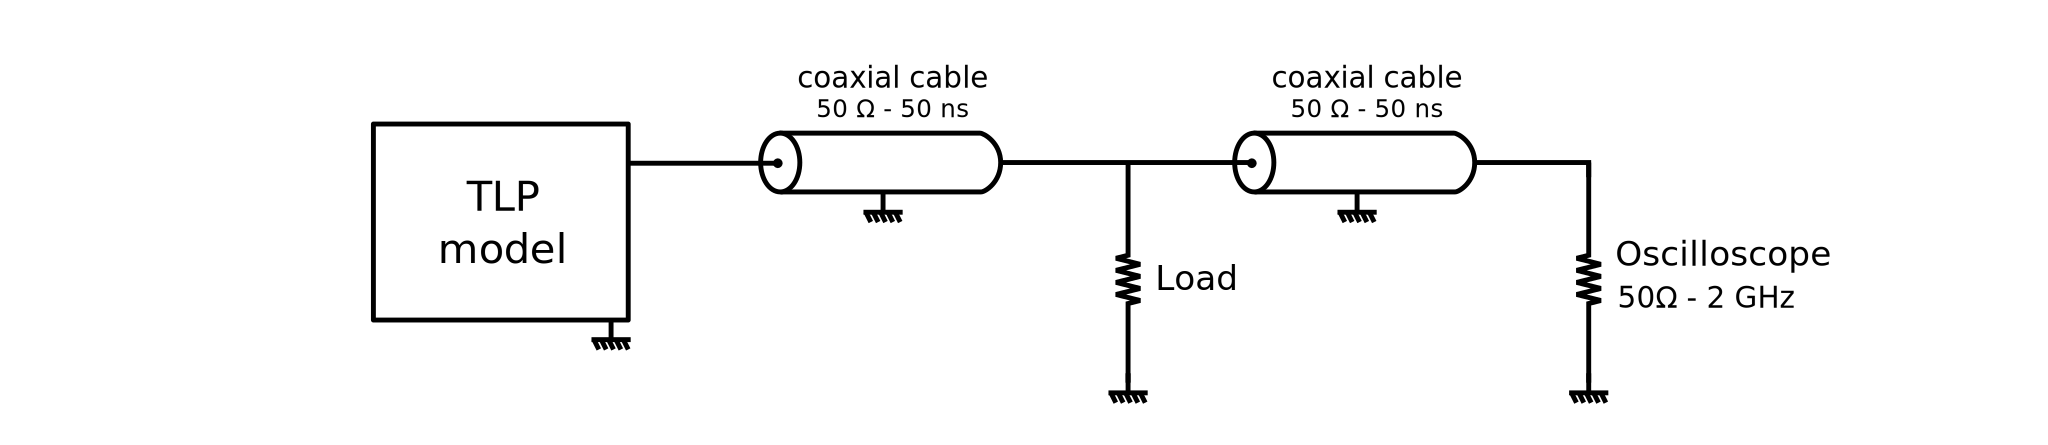
\includegraphics[width=\textwidth]{src/2/figures/tlp_characterization_setup.pdf}
  \caption{Characterization setup of the TLP}
  \label{fig:setup-cz-tlp-model}
\end{figure}

First comparison in Fig. \ref{fig:comparison-tlp-1-v} and \ref{fig:comparison-tlp-1-i}.
A 25\textOmega{} resistor allows validating the model with voltage across the load and current flowing through it.
The correlation is good and so far the model is rather accurate.
The ratio of Vtlp/Itlp between 40 ns to 100 ns is equal to the load resistance 25\textOmega{}.

\begin{figure}[!h]
  \centering
  \includegraphics[width=0.3\textwidth]{src/2/figures/tlp_comparison_25ohm_voltage.png}
  \caption{Voltage measurement versus simulation - XX V charging voltage on XX\textOmega{}}
  \label{fig:comparison-tlp-1-v}
\end{figure}

\begin{figure}[!h]
  \centering
  \includegraphics[width=0.3\textwidth]{src/2/figures/tlp_comparison_25ohm_current.png}
  \caption{Current measurement versus simulation - XX V charging voltage on XX\textOmega{}}
  \label{fig:comparison-tlp-1-i}
\end{figure}

Same comparison is performed on a short circuit in Fig. \ref{fig:comparison-tlp-short-v} and Fig. \ref{fig:comparison-tlp-short-i}.
The goal is to test the extreme conditions where the model is going to be used.
As expected the voltage is null and the current is close to the maximum 10A supplied by the TLP (500 V through 50\textOmega{}).
The same issue with probe clamping happens now with both voltage and current at exactly -100V and -5A.

\begin{figure}[!h]
  \centering
  \includegraphics[width=0.3\textwidth]{src/2/figures/tlp_comparison_short_voltage.png}
  \caption{Voltage measurement versus simulation - XX V charging voltage on a short circuit}
  \label{fig:comparison-tlp-short-v}
\end{figure}

\begin{figure}[!h]
  \centering
  \includegraphics[width=0.3\textwidth]{src/2/figures/tlp_comparison_short_current.png}
  \caption{Current measurement versus simulation - XX V charging voltage on a short circuit}
  \label{fig:comparison-tlp-short-i}
\end{figure}

Finally, the process is repeated on an open circuit in Fig. X and Fig. X

After 50 ns, voltage and current are stable.
The voltage is 250V which corresponds to half the TLP charging voltage, and the current is close to 0A.
This is expected behavior for a high impedance load.

On the current response (bottom), between 100ns and 120ns there is a significant difference between measurement and simulation.
This is simply due to the current probe clamping the current at -1A, because it exceeds the measurable range.
Since it is simply a measurement error it is not modeled.

\begin{figure}[!h]
  \centering
  \includegraphics[width=0.3\textwidth]{src/2/figures/tlp_comparison_open_voltage.png}
  \caption{Voltage measurement versus simulation - XX V charging voltage on open circuit}
  \label{fig:comparison-tlp-1-v}
\end{figure}

\begin{figure}[!h]
  \centering
  \includegraphics[width=0.3\textwidth]{src/1/figures/tlp_comparison_open_current.png}
  \caption{Current measurement versus simulation - XX V charging voltage on open circuit}
  \label{fig:comparison-tlp-1-i}
\end{figure}

Finally, only resistive loads were tested
Using a capacitor as load allows validating the model with non-purely real impedance.
Between 40 ns and 100 ns, voltage and current are not stable because the capacitor is too big to be fully charged at half the TLP charging voltage.
Because the TLP is closer to a current source than a voltage source, the capacitor is charged up at almost constant current, and its voltage rises linearly.
The slope of this linear curve is directly related to the capacitor value.
By extrapolation it is possible to measure the capacitor value from the TLP curve ?

\begin{figure}[!h]
  \centering
  \includegraphics[width=0.3\textwidth]{src/1/figures/tlp_comparison_capa_voltage.png}
  \caption{Voltage measurement versus simulation - XX V charging voltage on a 4nF capacitor}
  \label{fig:comparison-tlp-capa-v}
\end{figure}

\begin{figure}[!h]
  \centering
  \includegraphics[width=0.3\textwidth]{src/1/figures/tlp_comparison_capa_current.png}
  \caption{Current measurement versus simulation - XX V charging voltage on 4nF capacitor}
  \label{fig:comparison-tlp-capa-i}
\end{figure}

More simulations were run to ensure the model performs correctly at different charging voltages, etc
Goal is to validate it at its nominal and boundary conditions
Curves are given in Annex XX
%TODO: Mettre courbes en annexe
Overall, model is good and fits very well the measurements.
